\begin{figure}[H]
\centering
\begin{annotatedFigure}
	{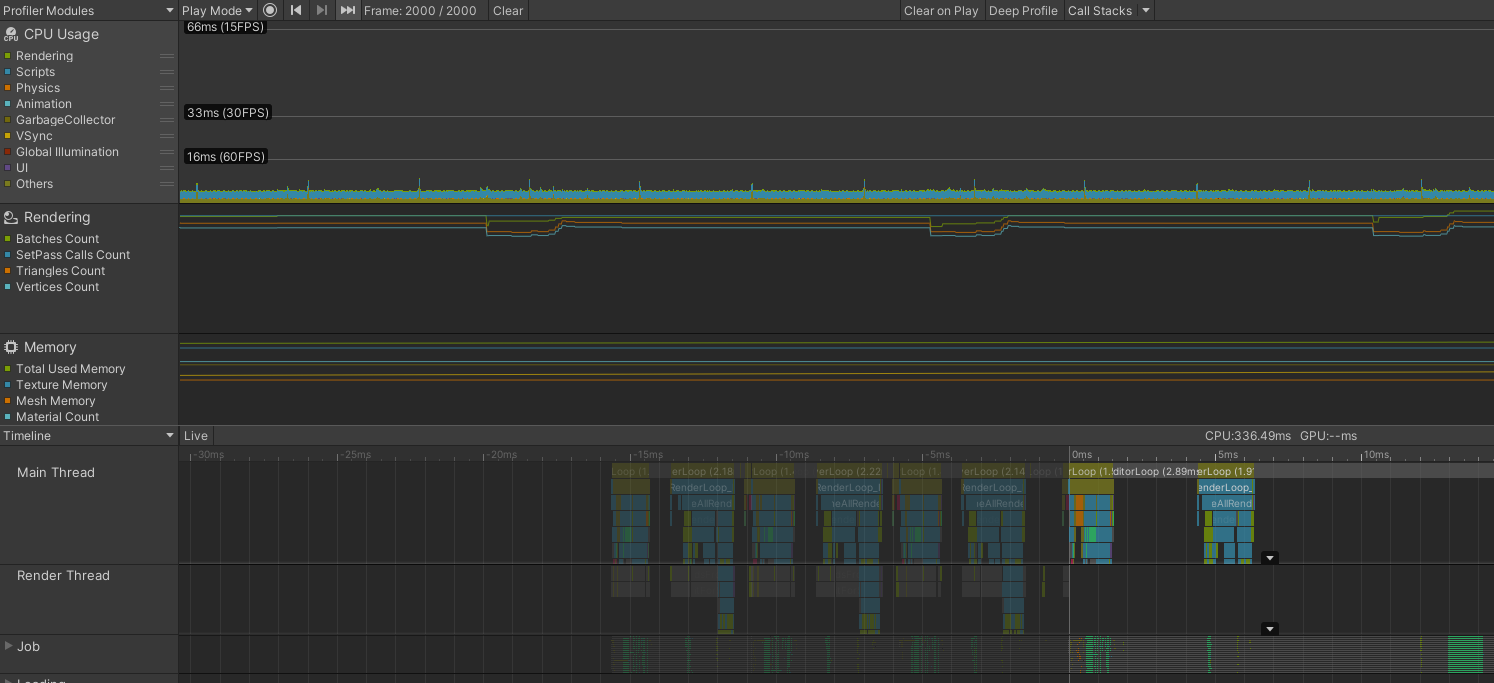
\includegraphics[scale=0.428]{Bilder/Profiler.png}}
    \annotatedFigureBox{0.1688,0.9496}{0.363,1.0039}{A}{0.363,0.9496}
	\annotatedFigureBox{0.125,0.6581}{1.013,0.7681}{B}{1.013,0.6581}
	\annotatedFigureBox{-0.011,0.3778}{0.1259,1.0016}{C}{0.1259,0.3778}
	\annotatedFigureBox{0.38,0.0888}{0.8705,0.3831}{D}{0.8705,0.0888}
\end{annotatedFigure}
\caption{Der Profiler in dem Unity Editor. Mit ihm lässt sich die Auslastung des Spiels während dem Spielen aufzeichnen und die Daten zur weiteren Verwendung abspeichern. Mit den Elementen bei A, lässt sich das Spiel wie gewünscht aufzeichnen und man sieht die Anzahl an aufgezeichneten Bildern. Mann kann auch einzelne Bilder auswählen. Bei B sieht man den Verlauf der aufgezeichneten Bilder. Hier sieht man für jedes Modul eine Auslastung über den Verlauf der 2000 Bildern. Bei C kann man die einzelnen Module sehen. Sichtbar sind hier die Module CPU Usage, Rendering und Memory, wobei man für weitere im Editor nach unten scrollen muss. Bei D ist eine genauere Timeline sichtbar, da hier nur einige Bilder abgebildet werden.}
\label{fig:profiler}
\end{figure}